\documentclass[t, 10pt, mathserif]{beamer}
% \usepackage{pgfpages}
% \pgfpagesuselayout{resize to}[a4paper,landscape,border shrink=5mm]
\usepackage[spanish]{babel}
\usepackage[utf8]{inputenc}
\usepackage{amscd}
\usepackage{amssymb}
\usepackage{amsthm}
\usepackage{latexsym}
\usepackage{setspace}
\usepackage{url}
\usepackage{xcolor}
\usepackage{bbm}

\mode<presentation>{
	\usecolortheme{}
	\useinnertheme{}
	\useoutertheme{}
}
\setbeamertemplate{sidebar right}{}
\setbeamertemplate{footline}{%
\hfill\usebeamertemplate***{navigation symbols}
\hspace{1cm}\insertframenumber{}/\inserttotalframenumber}

\beamertemplatenavigationsymbolsempty
\setbeamersize{text margin left = 1cm}
\setbeamertemplate{caption}[numbered]
\setbeamertemplate{frametitle}[default][left,leftskip=0.5cm]
\addtobeamertemplate{frametitle}{\vspace*{0.5cm}}{\vspace*{1cm}}

\setlength{\parskip}{\baselineskip}
\expandafter\def\expandafter\item\expandafter{\item \setlength{\parskip}{0.5\baselineskip}}

\languagepath{spanish}
\deftranslation[to=spanish]{Corollary}{Corolario}
\deftranslation[to=spanish]{corollary}{corolario}
\deftranslation[to=spanish]{Definition}{Definición}
\deftranslation[to=spanish]{definition}{definición}
\deftranslation[to=spanish]{Lemma}{Lema}
\deftranslation[to=spanish]{lemma}{lema}
\deftranslation[to=spanish]{Problem}{Problema}
\deftranslation[to=spanish]{problem}{problema}
\deftranslation[to=spanish]{Theorem}{Teorema}
\deftranslation[to=spanish]{theorem}{teorema}
\newtheorem{belief}{Belief}
\newtheorem{conjecture}{Conjecture}
\newtheorem{observation}{Observation}
\newtheorem{question}{Question}

\newcommand {\base}[2]{\langle{#1};{#2}\rangle}
\newcommand{\abs}[1]{\left| #1 \right|}
\newcommand{\alocc}[2]{|\!|#1|\!|_{#2}}
\newcommand{\card}{\mbox{\raisebox{.13em}{{$\scriptstyle \#$}}}}
\newcommand{\ceil}[1]{\lceil #1 \rceil }
\newcommand{\cf}{\text{\em cf}}
\newcommand{\eps}{\varepsilon}
\newcommand{\expa}[1]{\{#1\}}
\newcommand{\floor}[1]{\lfloor #1 \rfloor } 
\newcommand{\N}{{\mathbb{N}}}
\newcommand{\NN}{\mathbb{N}}
\newcommand{\occ}[2]{|#1|_{#2}}
\newcommand{\Q}{{\mathbb{Q}}}
\newcommand{\R}{{\mathbb{R}}}
\newcommand{\RR}{\mathbb{R}}
\newcommand{\uno}{\mathbbm{1}}
\newcommand{\wh}[1]{\widehat{#1}}
\newcommand{\xbar}{{\overline{x}}}
\newcommand{\ybar}{{\overline{y}}}
\newcommand{\Z}{{\mathbb{Z}}}

\author{\large Emilio Almansi}

\begin{document}

\title{\normalsize Tesis de Licenciatura en Ciencias de la Computación \vspace*{1.5cm}}

\subtitle{\Large Secuencias completamente equidistribuidas basadas en secuencias de De Bruijn}

\date{
  {\footnotesize
    \hspace*{-6cm}
    \begin{tabular}{l}
      Directora: Verónica Becher \\
      Departamento de Computación\\
      Facultad de Ciencias Exactas y Naturales\\
      Universidad de Buenos Aires\\
      4 de septiembre, 2019
    \end{tabular}
  }
}

%%%%%%%%%%%%%%%%%%%%%%%%%%%%%%%%%%%%%%%%%%%%%%%%%%%%%%%%%%%%%%%%%%%

\begin{frame}
  \vspace{0.5cm}
  \maketitle
  \setcounter{framenumber}{0}
  \thispagestyle{empty}
\end{frame}

%%%%%%%%%%%%%%%%%%%%%%%%%%%%%%%%%%%%%%%%%%%%%%%%%%%%%%%%%%%%%%%%%%%

\begin{frame}
  \frametitle{Sobre secuencias aleatorias {$^{(1)}$}}

  ¿Qué tienen en común las siguientes áreas?
  \pause

  \begin{itemize}
    \item Criptografía, seguridad informática.\pause
    \item Predicción del clima, medicina nuclear, simulación de proteínas.\pause
    \item Aprendizaje automático, algoritmos probabilistas.\pause
    \item Juegos de azar, videojuegos, simulaciones físicas.
  \end{itemize}
  \pause

  {\color{cyan} Generación de números aleatorios.}
  \pause

  Pero, ¿qué es una secuencia de números aleatorios?
\end{frame}

%%%%%%%%%%%%%%%%%%%%%%%%%%%%%%%%%%%%%%%%%%%%%%%%%%%%%%%%%%%%%%%%%%%

\begin{frame}
  \frametitle{Sobre secuencias aleatorias {$^{(2)}$}}

  \textbf{Intuición}: si tiro un dado muchas veces seguidas, el resultado de cada tirada tiene que ser \textit{impredecible} y todo número del 1 al 6 tiene que ser \textit{equiprobable}.
  \pause

  Respecto a la parte de \textit{impredecible}:
  \begin{quote}
    If ``random`` means that the sequence satisfies no predictable rules, the title of this paper is contradictory.
    \begin{flushright}
      \small{Construction of a Random Sequence \\}
      \small{Donald Knuth, 1965}
    \end{flushright}
  \end{quote}
  \pause

  En este trabajo, nos enfocamos en la parte de \textit{equiprobable}.
  % Es posible construir secuencias determinísticas que cumplen con esta propiedad.
\end{frame}

%%%%%%%%%%%%%%%%%%%%%%%%%%%%%%%%%%%%%%%%%%%%%%%%%%%%%%%%%%%%%%%%%%%

\begin{frame}
  \frametitle{Equidistribución {$^{(1)}$}}

  Dado un entero $b \ge 2$, una secuencia de \textit{números enteros} $X = x_1, x_2, \dots$ del conjunto $\{ 0, 1, \dots, b - 1 \}$ es \textbf{equidistribuida} si todo valor posible aparece con la misma frecuencia asintótica:
  \pause

  \begin{equation*}
    \begin{aligned}
      Pr \left( x_i = j \right) = \frac{1}{b} \hspace*{1cm} \text{para todo } j \in \{ 0, \dots, b - 1 \} \text{,}
    \end{aligned}
  \end{equation*}
  \pause

  \vspace{-0.5cm}
  donde $\displaystyle Pr(x_i = j) = \lim_{N \to \infty} \frac{1}{N} \sum_{i = 1}^{N} \sigma(x_i = j)$.
  \pause

  Ahora, damos una noción equivalente para secuencias de números reales.
\end{frame}

%%%%%%%%%%%%%%%%%%%%%%%%%%%%%%%%%%%%%%%%%%%%%%%%%%%%%%%%%%%%%%%%%%%

\begin{frame}
  \frametitle{Equidistribución {$^{(2)}$}}

  Una secuencia de \textit{números reales} $X = x_1, x_2, \dots$ en el intervalo unitario $\left[0, 1\right)$ es \textbf{equidistribuida} si, dado cualquier conjunto $I \subseteq \left[0, 1\right)$, la frecuencia asintótica con la que la secuencia toma valores en $I$ es igual a su tamaño:
  \pause

  \begin{equation*}
    \begin{aligned}
      Pr \left( x_i \in I\, \right) = \left| I\, \right| \hspace*{1cm} \text{para todo } I \subseteq \left[0, 1\right) \text{,}
    \end{aligned}
  \end{equation*}
  \pause

  \vspace{-0.5cm}
  donde $\displaystyle Pr \left( x_i \in I\, \right) = \lim_{N \to \infty} \frac{1}{N} \sum_{i = 1}^{N} \sigma(x_i \in I\,)$.
  \pause

  Si $X$ es equidistribuida en $[0, 1)$, entonces para cualquier $b \ge 2$ la secuencia $Y = \lfloor b x_1 \rfloor, \lfloor b x_2 \rfloor, \dots$ es equidistribuida en $\{ 0, 1, \dots, b - 1 \}$.
\end{frame}

%%%%%%%%%%%%%%%%%%%%%%%%%%%%%%%%%%%%%%%%%%%%%%%%%%%%%%%%%%%%%%%%%%%

\begin{frame}
  \frametitle{Equidistribución {$^{(3)}$}}

  \vspace{1cm}
  \begin{figure}
    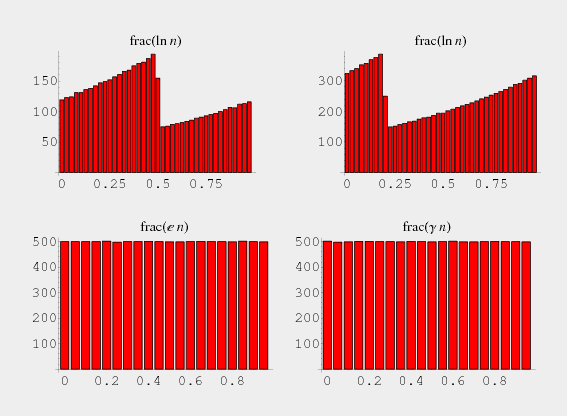
\includegraphics[scale=0.4]{resources/equidistribucion.png}
    \caption{Secuencias de partes fraccionarias.}
  \end{figure}
\end{frame}
 
%%%%%%%%%%%%%%%%%%%%%%%%%%%%%%%%%%%%%%%%%%%%%%%%%%%%%%%%%%%%%%%%%%%

\begin{frame}
  \frametitle{$k$-distribución {$^{(1)}$}}

  % Ahora extendemos la noción de equidistribución a otras dimensiones.
  % \pause

  \textbf{Intuición}: cualquier seguidilla de tiradas tiene que aparecer con igual frecuencia. Por ejemplo, (1, 2, 3) aparece con la misma frecuencia que (3, 2, 1) y que (6, 6, 6).
  \pause

  Trabajamos con ``ventanas`` de tamaño $k$ de la secuencia. Si $X = x_1, x_2, \dots$ es una secuencia de \textit{números reales}, entonces:
  \pause

  \vspace{-0.3cm}
  \begin{equation*}
    \begin{aligned}
        \bar{w}_1 & = (x_1, x_2, \dots, x_k      ), \\
        \bar{w}_2 & = (x_2, x_3, \dots, x_{k + 1}), \\
        \bar{w}_3 & = (x_3, x_4, \dots, x_{k + 2}), \\
            & \dots
    \end{aligned}
  \end{equation*}

  es la secuencia de ventanas de $X$, que llamamos $W_k(X)$.
\end{frame}

%%%%%%%%%%%%%%%%%%%%%%%%%%%%%%%%%%%%%%%%%%%%%%%%%%%%%%%%%%%%%%%%%%%

\begin{frame}
  \frametitle{$k$-distribución {$^{(2)}$}}

  Una secuencia de \textit{números reales} $X = x_1, x_2, \dots$ en el intervalo unitario $\left[0, 1\right)$ es \textbf{$k$-distribuida} si, dado cualquier conjunto $I \subseteq \left[0, 1\right)^k$, la frecuencia asintótica con la que la secuencia de ventanas de $X$ toma valores en $I$ es igual a su tamaño:
  \pause

  \begin{equation*}
    \begin{aligned}
      Pr \left( \bar{w}_i \in I\, \right) = \left| I\, \right| \hspace*{1cm} \text{para todo } I \subseteq \left[0, 1\right)^k \text{,}
    \end{aligned}
  \end{equation*}
  \pause

  \vspace{-0.5cm}
  \begin{equation*}
    \hspace{-2.5cm}
    \begin{aligned}
        \text{donde } W_k(X) =\; & \bar{w}_1, \bar{w}_2, \dots \\
                              =\; & (x_1, x_2, \dots, x_k      ),\, (x_2, x_3, \dots, x_{k + 1}),\, \dots \, \text{.}
    \end{aligned}
  \end{equation*}
  \vspace{-0.3cm}
  \pause

  Si $X$ es $k$-distribuida para todo $k$, entonces $X$ es \textbf{completamente equidistribuida}.
\end{frame}

%%%%%%%%%%%%%%%%%%%%%%%%%%%%%%%%%%%%%%%%%%%%%%%%%%%%%%%%%%%%%%%%%%%

\begin{frame}
  \frametitle{Equidistribución completa {$^{(1)}$}}

  ¿Por qué estudiar la propiedad de equidistribución?

  \begin{itemize}
    \item Requerimiento básico de pseudo-aleatoriedad. Propiedades de equipartición y autocorrelación con retraso. \pause
    \item Calidad de un generador de números aleatorios o PRNG. Pruebas de aleatoriedad.\pause % Mersenne Twister
    \item Integración de Montecarlo, criterio de la integral de Riemann. \pause
    \item Vínculo: teoría de números, computación, probabilidad y estadística.
  \end{itemize}
  \pause

  ¿Qué \textbf{no} es la equidistribución?
\end{frame}
 
%%%%%%%%%%%%%%%%%%%%%%%%%%%%%%%%%%%%%%%%%%%%%%%%%%%%%%%%%%%%%%%%%%%

\begin{frame}
  \frametitle{Equidistribución completa {$^{(2)}$}}

  \vspace{0.5cm}
  \begin{figure}
    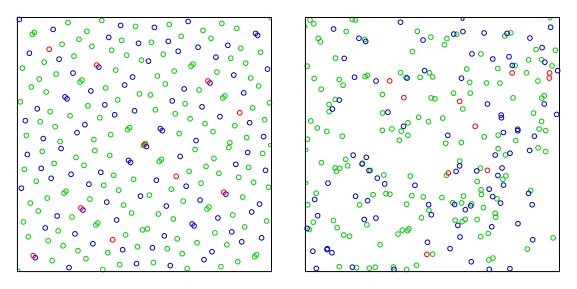
\includegraphics[width=0.6\textwidth]{resources/discrepancia.png}
    \caption{Izq.) Sec. pseudo-aleatoria Der.) Sec. Sobol 2,3. }
  \end{figure}
\end{frame}
 
%%%%%%%%%%%%%%%%%%%%%%%%%%%%%%%%%%%%%%%%%%%%%%%%%%%%%%%%%%%%%%%%%%%

\begin{frame}{Secuencias de De Bruijn}
  \only<1->{
    Son secuencias muy estudiadas en combinatoria. Una secuencia $b$-aria de De Bruijn de orden $k$ ``contiene`` a cada posible secuencia $b$-aria de longitud $k$ exactamente una vez. Ejemplos:
  }

  \only<1->{Con $b = 2, k = 3$:}
  \only<2->{\vspace{-0.3cm}}
  \begin{center}
    \only<2>{$0, 0, 0, 1, 0, 1, 1, 1$}
    \only<3>{$\textbf{0, 0, 0}, 1, 0, 1, 1, 1$}
    \only<4>{$0, \textbf{0, 0, 1}, 0, 1, 1, 1$}
    \only<5>{$0, 0, \textbf{0, 1, 0}, 1, 1, 1$}
    \only<6>{$0, 0, 0, \textbf{1, 0, 1}, 1, 1$}
    \only<7>{$0, 0, 0, 1, \textbf{0, 1, 1}, 1$}
    \only<8>{$0, 0, 0, 1, 0, \textbf{1, 1, 1}$}
    \only<9>{$\textbf{0}, 0, 0, 1, 0, 1, \textbf{1, 1}$}
    \only<10>{$\textbf{0, 0}, 0, 1, 0, 1, 1, \textbf{1}$}
    \only<11->{$0, 0, 0, 1, 0, 1, 1, 1$}
    \only<11->{\vspace{-0.3cm}}
  \end{center}

  \only<11->{Con $b = 4, k = 2$:}
  \only<11->{\vspace{-0.3cm}}
  \begin{center}
    \only<12->{$0, 0, 1, 0, 2, 0, 3, 1, 1, 2, 1, 3, 2, 2, 3, 3$}
  \end{center}

  \only<13->{Notar que siempre tienen longitud $b^k$.}
  \only<14->{{\color{cyan} ¿Qué relación tienen con las secuencias equidistribuidas?}}
\end{frame}

%%%%%%%%%%%%%%%%%%%%%%%%%%%%%%%%%%%%%%%%%%%%%%%%%%%%%%%%%%%%%%%%%%%

\begin{frame}
  \frametitle{Secuencia de Knuth {$^{(1)}$}}
  \pause

  \vspace{-0.5cm}
  \begin{definition}
    \medskip
    Una \textbf{secuencia $A$ de orden $n$} es la secuencia que se obtiene al dividir cada elemento de una secuencia $2^n$-aria de De Bruijn de orden $n$ por $2^n$:
    \pause

    \begin{equation*}
      \begin{aligned}
        A^{(n)} & = \frac{x_1}{2^n}, \frac{x_2}{2^n}, \dots, \frac{x_{2^{n^2}}}{2^n}
      \end{aligned}
    \end{equation*}

    \medskip
    donde $x_1, \dots, x_{2^{n^2}}$ es una secuencia $2^n$-aria de De Bruijn de orden $n$.
  \end{definition}
  \pause

  \begin{definition}
    \medskip
    Una \textbf{secuencia $B$ de orden $n$} es la secuencia que se obtiene de concatenar $n 2^{2 n}$ copias de una secuencia $A$ de orden $n$:
    \pause

    \begin{equation*}
      B^{(n)} = \left< \underbrace{A^{(n)} ; A^{(n)} ; \dots ; A^{(n)}}_{n 2^{2 n} \text{ veces}} \right> \text{.}
    \end{equation*}
  \end{definition}
\end{frame}


%%%%%%%%%%%%%%%%%%%%%%%%%%%%%%%%%%%%%%%%%%%%%%%%%%%%%%%%%%%%%%%%%%%

\begin{frame}
  \frametitle{Secuencia de Knuth {$^{(2)}$}}

  Ejemplo para $n = 2$:
  \pause

  \begin{equation*}
    \begin{aligned}
      X^{(4, 2)} & = 0, 0, 1, 0, 2, 0, 3, 1, 1, 2, 1, 3, 2, 2, 3, 3 \text{;} \\[0.4cm] \pause
      A^{(2)}    & = \frac{0}{4}, \frac{0}{4}, \frac{1}{4}, \frac{0}{4}, \frac{2}{4}, \frac{0}{4}, \frac{3}{4}, \frac{1}{4}, \frac{1}{4}, \frac{2}{4}, \frac{1}{4}, \frac{3}{4}, \frac{2}{4}, \frac{2}{4}, \frac{3}{4}, \frac{3}{4} \text{;} \\[0.4cm] \pause
      B^{(2)}   & = \left< \underbrace{A^{(2)} ; \dots ; A^{(2)}}_{2 \times 2^{2 \times 2} = 32 \text{ veces}} \right> \\[0.1cm] \pause
                & = \underbrace{\frac{0}{4}, \frac{0}{4}, \dots, \frac{3}{4}, \frac{3}{4}}_{A^{(2)}}, \dots, \underbrace{\frac{0}{4}, \frac{0}{4}, \dots, \frac{3}{4}, \frac{3}{4}}_{A^{(2)}} \text{.}
    \end{aligned}
  \end{equation*}
\end{frame}

%%%%%%%%%%%%%%%%%%%%%%%%%%%%%%%%%%%%%%%%%%%%%%%%%%%%%%%%%%%%%%%%%%%

\begin{frame}
  \frametitle{Secuencia de Knuth {$^{(3)}$}}

  Ahora sí ya estamos en condiciones de definir la secuencia de Knuth.
  \pause

  \medskip
  \begin{definition}[{{\scriptsize  Knuth, 1965}}]
    \medskip
    La secuencia de Knuth, que denominamos $K$, se define como la concatenación de las secuencias $B^{(n)}$ para $n = 1, 2, 3, \dots$:
    \pause

    \begin{equation*}
      K = \left< B^{(1)} ; B^{(2)} ;  B^{(3)} ; \dots \right> \text{.}
    \end{equation*}
  \end{definition}
  \pause

  \medskip
  \begin{theorem}[{{\scriptsize  Knuth, 1965}}]
    \medskip
    La secuencia $K$ es completamente equidistribuida.
  \end{theorem}
\end{frame}

%%%%%%%%%%%%%%%%%%%%%%%%%%%%%%%%%%%%%%%%%%%%%%%%%%%%%%%%%%%%%%%%%%%

\begin{frame}{Secuencia de Knuth {$^{(4)}$}}
  \only<1>{
    \begin{figure}
      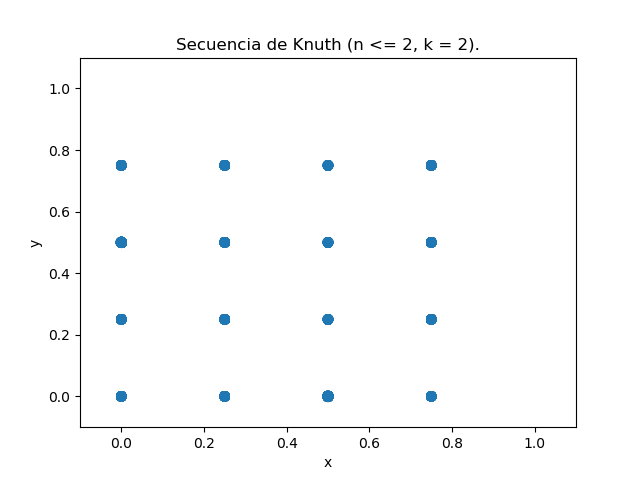
\includegraphics[width=0.6\textwidth]{resources/secuencia-knuth-1.png}
      \caption{Secuencia de Knuth en dos dimensiones.}
    \end{figure}
  }
  \only<2>{
    \begin{figure}
      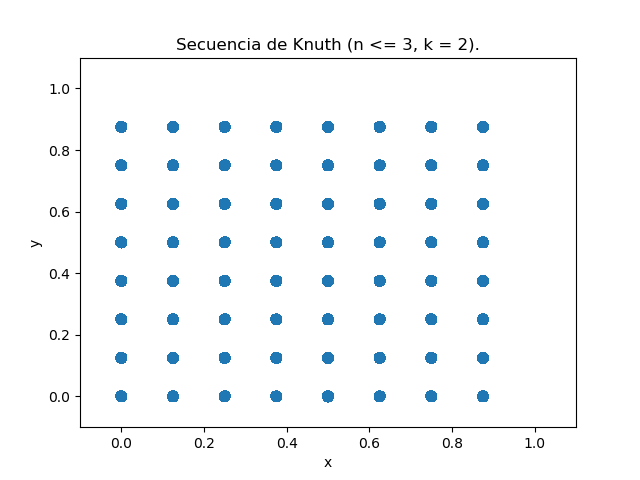
\includegraphics[width=0.6\textwidth]{resources/secuencia-knuth-2.png}
      \caption{Secuencia de Knuth en dos dimensiones.}
    \end{figure}
  }
\end{frame}
 
%%%%%%%%%%%%%%%%%%%%%%%%%%%%%%%%%%%%%%%%%%%%%%%%%%%%%%%%%%%%%%%%%%%

\begin{frame}
  \frametitle{Comentarios sobre la demostración}

  Knuth da una prueba elemental de este teorema.
  \pause
  
  Dos decisiones en la construcción de $K$ parecen arbitrarias, pero juegan un rol importante en la demostración:
  \pause

  \begin{itemize}
    \item La cantidad $n 2^{2n}$ de repeticiones de una secuencia $A$ en una secuencia $B$. \pause
    % On account of the first choice, one can adapt Knuth's proof in a rather straightforward manner to show that a sufficient condition for the complete equidistribution of $K$ is for the number of repetitions to grow asymptotically faster than $2^{2n}$. A proof of this fact is omitted here since it follows from Knuth's work, together with the technique used in the following section to obtain an analogous result. Knuth's choice of $n 2^{2n}$ repetitions is sufficient to achieve complete equidistribution, but a more reduced number of repetitions such as $\lceil \log(n + 1) \rceil 2^{2n}$ would suffice as well.
  
    \item El uso de secuencias de De Bruijn $2^n$-arias de orden $n$.
    % In regard to the second choice, Knuth's use of alphabet sizes which grow exponentially as powers of $2$ allows one to reason more easily about the rational numbers comprised in the sequence $K$ in terms of their binary representations. In particular, Knuth uses this device to derive properties of the distribution of the $m$ most-significant bits of the terms in a $2^n$-ary Ford sequence, where $m \le n$. See \cite[Lemma 2]{knuth-1965}.

  \end{itemize}
  \pause

  Si usamos secuencias de De Bruijn con alfabetos que crecen linealmente en tamaño, {\color{cyan}¿sigue siendo completamente equidistribuida la secuencia? ¿Cuántas repeticiones son necesarias?}
\end{frame}

%%%%%%%%%%%%%%%%%%%%%%%%%%%%%%%%%%%%%%%%%%%%%%%%%%%%%%%%%%%%%%%%%%%

\begin{frame}
  \frametitle{Alfabetos linealmente crecientes {$^{(1)}$}}
  \pause

  \vspace{-0.5cm}
  \begin{definition}
    \medskip
    Una \textbf{secuencia $C$ de orden $n$} es la secuencia que se obtiene al dividir cada elemento de una secuencia $n$-aria de De Bruijn de orden $n$ por $n$:
    \pause

    \begin{equation*}
      \begin{aligned}
        C^{(n)} & = \frac{x_1}{n}, \frac{x_2}{n}, \dots, \frac{x_{n^n}}{n}
      \end{aligned}
    \end{equation*}

    \medskip
    donde $x_1, \dots, x_{n^n}$ es una secuencia $n$-aria de De Bruijn de orden $n$.
  \end{definition}
  \pause

  \begin{definition}
    \medskip
    Dada $t : \mathbb{N} \mapsto \mathbb{N}$, una \textbf{secuencia $D$ de orden $n$} es la secuencia que se obtiene de concatenar $t(n)$ copias de una secuencia $C$ de orden $n$:
    \pause

    \begin{equation*}
      D^{(n, t)} = \left< \underbrace{C^{(n)} ; C^{(n)} ; \dots ; C^{(n)}}_{t(n) \text{ veces}} \right> \text{.}
    \end{equation*}
  \end{definition}
\end{frame}

%%%%%%%%%%%%%%%%%%%%%%%%%%%%%%%%%%%%%%%%%%%%%%%%%%%%%%%%%%%%%%%%%%%

\begin{frame}
  \frametitle{Alfabetos linealmente crecientes {$^{(1)}$}}

  \vspace{-0.5cm}
  \begin{definition}
    \medskip
    Una \textbf{secuencia $C$ de orden $n$} es la secuencia que se obtiene al dividir cada elemento de una secuencia {\color{cyan} $n$-aria} de De Bruijn de orden $n$ por {\color{cyan} $n$}:

    \begin{equation*}
      \begin{aligned}
        C^{(n)} & = \frac{x_1}{{\color{cyan} n}}, \frac{x_2}{{\color{cyan} n}}, \dots, \frac{x_{{\color{cyan} n^n}}}{{\color{cyan} n}}
      \end{aligned}
    \end{equation*}

    \medskip
    donde $x_1, \dots, x_{{\color{cyan} n^n}}$ es una secuencia {\color{cyan} $n$-aria} de De Bruijn de orden $n$.
  \end{definition}

  \begin{definition}
    \medskip
    Dada ${\color{cyan} t : \mathbb{N} \mapsto \mathbb{N}}$, una \textbf{secuencia $D$ de orden $n$} es la secuencia que se obtiene de concatenar ${\color{cyan} t(n)}$ copias de una secuencia $C$ de orden $n$:

    \begin{equation*}
      D^{(n, {\color{cyan} t})} = \left< \underbrace{C^{(n)} ; C^{(n)} ; \dots ; C^{(n)}}_{{\color{cyan} t(n)} \text{ veces}} \right> \text{.}
    \end{equation*}
  \end{definition}
\end{frame}

%%%%%%%%%%%%%%%%%%%%%%%%%%%%%%%%%%%%%%%%%%%%%%%%%%%%%%%%%%%%%%%%%%%

\begin{frame}
  \frametitle{Alfabetos linealmente crecientes {$^{(2)}$}}

  Ejemplo para $n = 3$, $t(n) = n$:
  \pause

  \begin{equation*}
    \begin{aligned}
      X^{(3, 3)} & = 0, 0, 0, 1, 0, 0, 2, 0, 1, 1, 0, 1, 2, 0, 2, 1, 0, 2, 2, 1, 1, 1, 2, 1, 2, 2, 2  \text{;} \\[0.4cm] \pause
      C^{(3)}    & = \frac{0}{3}, \frac{0}{3}, \frac{0}{3}, \frac{1}{3}, \frac{0}{3}, \frac{0}{3}, \frac{2}{3}, \frac{0}{3}, \frac{1}{3}, \frac{1}{3}, \frac{0}{3}, \frac{1}{3}, \frac{2}{3}, \frac{0}{3}, \\[0.2cm]
                 & \hspace{0.5cm} \frac{0}{3}, \frac{2}{3}, \frac{1}{3}, \frac{0}{3}, \frac{2}{3}, \frac{2}{3}, \frac{1}{3}, \frac{1}{3}, \frac{1}{3}, \frac{2}{3}, \frac{1}{3}, \frac{2}{3}, \frac{2}{3}, \frac{2}{3} \text{;} \\[0.4cm] \pause
      D^{(3)}   & = \underbrace{\frac{0}{3}, \frac{0}{3}, \dots, \frac{2}{3}, \frac{2}{3}}_{C^{(3)}}, \underbrace{\frac{0}{3}, \frac{0}{3}, \dots, \frac{2}{3}, \frac{2}{3}}_{C^{(3)}}, \underbrace{\frac{0}{3}, \frac{0}{3}, \dots, \frac{2}{3}, \frac{2}{3}}_{C^{(3)}} \text{.}
    \end{aligned}
  \end{equation*}
\end{frame}

%%%%%%%%%%%%%%%%%%%%%%%%%%%%%%%%%%%%%%%%%%%%%%%%%%%%%%%%%%%%%%%%%%%

\begin{frame}
  \frametitle{Secuencia $L$ {$^{(1)}$}}

  \begin{definition}[Esta tesis]
    \medskip
    Dada $t : \mathbb{N} \mapsto \mathbb{N}$, la secuencia $L^{(t)}$ se define como la concatenación de las secuencias $D^{(n, t)}$ para $n = 1, 2, 3, \dots$:
    \pause

    \begin{equation*}
      L^{(t)} = \left< D^{(1, t)} ; D^{(2, t)} ;  D^{(3, t)} ; \dots \right> \text{.}
    \end{equation*}
  \end{definition}
  \pause

  {\color{cyan} Ahora, enunciamos el aporte principal de esta tesis.}
  \pause

  \medskip
  \begin{block}{Teorema 1}
    \medskip
    \textit{Si $t : \mathbb{N} \mapsto \mathbb{N}$ es una función no decreciente y $\lim_{n \to \infty} n / t(n) = 0$, entonces la secuencia $L^{(t)}$ es completamente equidistribuida.}
  \end{block}
\end{frame}

%%%%%%%%%%%%%%%%%%%%%%%%%%%%%%%%%%%%%%%%%%%%%%%%%%%%%%%%%%%%%%%%%%%

\begin{frame}{Secuencia $L$ {$^{(2)}$}}
  \only<1>{
    \begin{figure}
      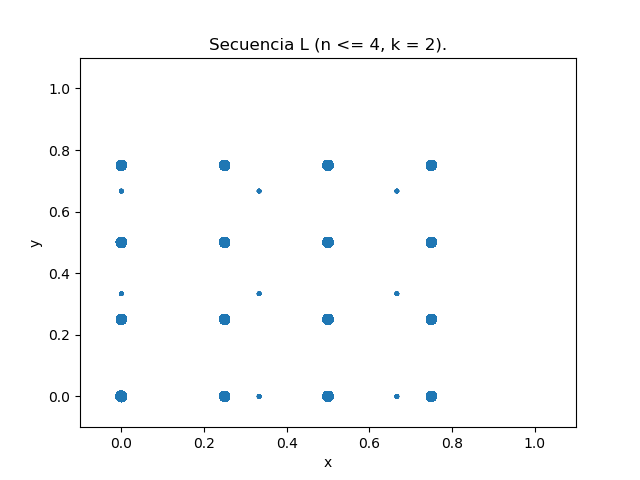
\includegraphics[width=0.6\textwidth]{resources/secuencia-l-1.png}
      \caption{Secuencia $L^{(t)}$ con $t(n) = n^2$ en dos dimensiones.}
    \end{figure}
  }
  \only<2>{
    \begin{figure}
      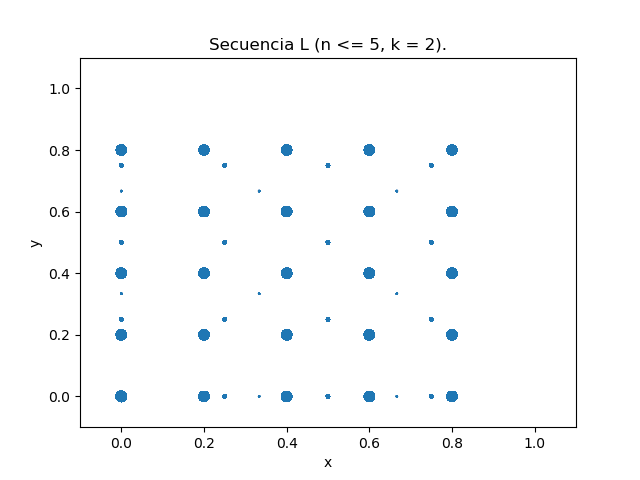
\includegraphics[width=0.6\textwidth]{resources/secuencia-l-2.png}
      \caption{Secuencia $L^{(t)}$ con $t(n) = n^2$ en dos dimensiones.}
    \end{figure}
  }
\end{frame}
 
%%%%%%%%%%%%%%%%%%%%%%%%%%%%%%%%%%%%%%%%%%%%%%%%%%%%%%%%%%%%%%%%%%%

\begin{frame}
  \frametitle{Idea de la demostración {$^{(1)}$}}

  Recordando la definición, queremos probar que para cualquier $k$ vale:

  \vspace{-0.5cm}
  \begin{equation*}
    \begin{aligned}
      Pr \left( \bar{w}_i \in I\, \right) = \left| I\, \right| \hspace*{1cm} \text{para todo } I \subseteq \left[0, 1\right)^k \text{,}
    \end{aligned}
  \end{equation*}
  
  donde $W_k(L) = \bar{w}_1, \bar{w}_2, \dots$ es la secuencia de ventanas de orden $k$ de $L$.
  \pause

  Queremos contar cuántas ventanas $\bar{w}_i$ caen adentro de un $I$ arbitrario.
  \pause

  Pensemos en los primeros $N$ elementos de la secuencia $L$. Este prefijo $L_{1:N}$ se puede partir en cuatro partes:
  \pause

  \begin{equation*}
    L_{1:N} = \left< S^{(1)} ; S^{(2)} ; S^{(3)} ; S^{(4)} \right>
  \end{equation*}
  
\end{frame}

%%%%%%%%%%%%%%%%%%%%%%%%%%%%%%%%%%%%%%%%%%%%%%%%%%%%%%%%%%%%%%%%%%%

\begin{frame}
  \frametitle{Idea de la demostración {$^{(2)}$}}

  Calculamos cuántas ventanas pertenecen a $I$ en cada parte. Después sumamos, dividimos por $N$, y tomamos el límite. El resultado es $Pr \left( \bar{w}_i \in I\, \right)$.
  \pause

  Para las partes $S^{(1)}$ y $S^{(4)}$, podemos acotar la cantidad de ventanas por la longitud del segmento. Para las partes $S^{(2)}$ y $S^{(3)}$, necesitamos el siguiente lema:
  \pause

  \begin{lemma}
    \medskip
    Dado un entero positivo $k$ y un conjunto $I \subseteq [0, 1)^k$, sea $n \in \mathbb{N}$ tal que $k \le n$. Luego, para algún $\varepsilon \in (-1, 1)$:
    \begin{equation*}
      \sum_{i = 1}^{n^n} \sigma\Big( \big( W_k^{c}(C^{(n)}) \big)_i \in I \Big) = n^n |I| + n^{n - 1} (2^k - 1) \varepsilon \text{.}
    \end{equation*}
  \end{lemma}

\end{frame}

%%%%%%%%%%%%%%%%%%%%%%%%%%%%%%%%%%%%%%%%%%%%%%%%%%%%%%%%%%%%%%%%%%%

\begin{frame}
  \frametitle{Comentarios sobre la demostración}

  La prueba de Knuth usa la propiedad de que los denominadores son potencias de $2$. Con el lema previo, podemos hacer la cuenta para cualquier denominador arbitrario.
  \pause

  Transformamos los números racionales en $C^{(n)}$ a enteros. La condición $\bar{w_i} \in I$ se transforma en un sistema de inecuaciones. Podemos contar la cantidad de soluciones dentro de $C^{(n)}$ gracias a la propiedad de De Bruijn.
  \pause

  Las condiciones sobre $t$ surgen como medio para garantizar que el límite sobre la parte $S^{(4)}$ se vaya a $0$.
  \pause

  También damos una prueba alternativa más sencilla, aunque no es elemental ya que se basa en el criterio de Weyl.

\end{frame}

% %%%%%%%%%%%%%%%%%%%%%%%%%%%%%%%%%%%%%%%%%%%%%%%%%%%%%%%%%%%%%%%%%%%

% \begin{frame}
%   \frametitle{Prueba alternativa {$^{(1)}$}}

%   También damos una prueba alternativa más sencilla, aunque no es elemental ya que se basa en el criterio de Weyl.
%   \pause

%   \medskip
%   \begin{block}{Criterio de Weyl}
%     \medskip
%     Una secuencia $X = x_1, x_2, \dots$ de números reales en $[0, 1)$ es $k$-distribuida si, y solo si, para cualquier vector de enteros no nulo $\bar{\ell} = (l_1, \dots, l_k)$:
%     \pause

%     \begin{equation*}
%       \lim_{N \to \infty} \frac{1}{N} \sum_{n = 1}^{N} e^{2 \pi i \bar{\ell} \cdot \bar{w}_n} = 0 \text{,}
%     \end{equation*}

%     donde $W_k(X) = \bar{w}_1, \bar{w}_2, \dots$ es la secuencia de ventanas de orden $k$ de $X$.
%   \end{block}
%   \pause

%   Podemos reducir el problema a una cota sobre una suma exponencial.
% \end{frame}

% %%%%%%%%%%%%%%%%%%%%%%%%%%%%%%%%%%%%%%%%%%%%%%%%%%%%%%%%%%%%%%%%%%%

% \begin{frame}
%   \frametitle{Prueba alternativa {$^{(2)}$}}

%   Mauris euismod neque a lorem rutrum, id molestie eros consequat.
%   \pause
  
%   In facilisis magna eu libero commodo, id tincidunt {\color{magenta} $\ell$} purus pellentesque.
%   \pause

%   \medskip
%   \begin{definition}
%     Fusce sit amet lacus viverra, viverra massa sit amet, placerat neque. Integer ipsum sapien, efficitur quis dui vitae, facilisis tempus dolor.
%     \pause

%     Duis ornare volutpat libero, at sodales dolor porttitor at.
%     \pause
%   \end{definition}

%   In rutrum dapibus justo, at mattis lacus ultrices sed. Suspendisse suscipit luctus fermentum.
% \end{frame}

%%%%%%%%%%%%%%%%%%%%%%%%%%%%%%%%%%%%%%%%%%%%%%%%%%%%%%%%%%%%%%%%%%%

\begin{frame}
  \frametitle{Problemas abiertos}

  Líneas de investigación futura:
  \pause

  \begin{itemize}
    \item ¿Qué pasa cuando no se cumple que $\lim_{n \to \infty} n / t(n) = 0$? ¿La secuencia $L$ sigue siendo completamente equidistribuida? % Idem seq K. % Para responder eso, es necesario entender mejor la discrepancia de la secuencia $L$.
    \pause
    
    \item ¿Qué pasa si cambiamos las secuencias de De Bruijn por alguna de sus variantes?
    \pause

    \item Relacionado: ¿cumple la secuencia $L$ la propiedad de correlación de pares de Poisson?
  \end{itemize}
\end{frame}

%%%%%%%%%%%%%%%%%%%%%%%%%%%%%%%%%%%%%%%%%%%%%%%%%%%%%%%%%%%%%%%%%%%

\begin{frame}
  \frametitle{¿Preguntas?}

  \vspace{-0.5cm}
  \begin{figure}
    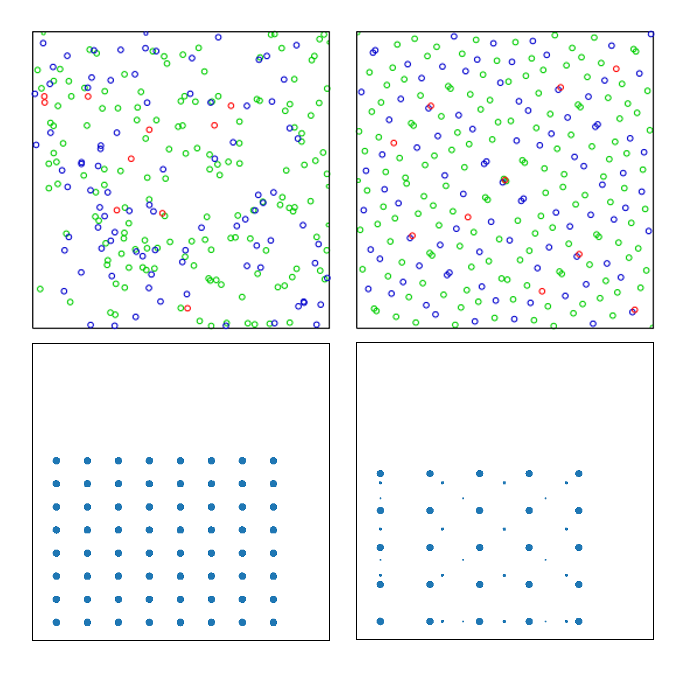
\includegraphics[scale=0.3]{resources/ultima.png}
    \caption{Secuencias $2$-distribuidas.}
  \end{figure}
\end{frame}
 
\end{document}
